
%%% Local Variables:
%%% mode: latex
%%% TeX-master: t
%%% End:

\chapter{样式使用说明}
\label{cha:command}


\section{引言(引言标题可选)}
\label{sec:cover}
华中科技大学学位论文格式要求。

\section{导入自定义功能区}
为了方便使用,\textbf{添加“插入题注”和“插入交叉引用”等常用功能到word快速访问工具栏。}

(1)下载文件“Word 自定义.exportedUI”

(2)点击“WORD-文件-选项-自定义功能区-导入导出”,将文件“Word 自定义.exportedUI”导入。


\section{奇数页放置}
不要随意删除分节符、分页符。

(1)摘要、目录奇数页放置

(2)各章首页可以连续放置,需要加入分节符(下一页)

\section{各级标题}
输入文本内容,直接选择样式中对应的标题样式即可。

正文需要自定义手动添加二个字符缩进。


\section{图片表格自动编号与引用}
(1)制作图片或表格。

(2)点击图片或表格,选择样式“图标题”

(3)插入题注自动编号。题目推荐使用二个空格,不建议使用TAB空格(图目录不方便调节缩进)。

(4)交叉引用。在需要引用公式的地方用“插入”->“交叉引用”,选择引用类型和引用内容“只有标签和编号”交叉引用公式编号。如图\ref{Fig2-1}所示。

\begin{figure}[!htbp]
    \centering
    \includegraphics{Fig2-1}
    \caption{测试图标题}
    \label{Fig2-1}
\end{figure}
%\vspace{-2em}
可以从图中观察到,xxx。

\begin{figure}
	\subfloat[EDN-ARMOEA]{
        \begin{minipage}[t]{0.5\linewidth}
        \includegraphics[width=1\linewidth]{figures/Fig2-1.png}
        \label{fig1111}
        \end{minipage}%
        }
	\subfloat[EDN-ARMOEA]{
        \begin{minipage}[t]{0.5\linewidth}
        \includegraphics[width=1\linewidth]{figures/Fig2-1.png}
        \label{fig222}
        \end{minipage}
    }
    \label{fig333}
    \caption{asas}
\end{figure}

如图\ref{fig222}所示。

\section{公式的自动编号与引用}
举例:这里我们考虑一个由$N$个跟随者和一个编号为0的领导者$L_w = 150 m$构成的多自主体网络。其中,跟随者的动力学由如下动力学描述
\begin{equation}
\sum_{i=1}^{\left[ \frac{n}{2}\right]} \binom{x_{i,i+1}^{i^2}}
{\left[\frac{i+3}{3} \right]} \frac{\sqrt{\mu(i)^{\frac{3}{2}}
(i^2-1)}} {\sqrt[3]{\rho(i)-2}+\sqrt[3]{\rho(i)-1}}
\end{equation}
其中第$i$个自主体的状态$x_i (t)\in R$,f$(x_i (t))$代表非线性连续可微函数,$U_i$表示节点i的控制输入。


\section{三线表}
任意绘制一个表格,点击“表格工具-设计”,选中自定义样式“三线表”,即可套用。填入表格内容后,全选应用“题注”样式(居中,五号)。如表\ref{Tab2-1}和表\ref{Tab2-2}所示.表前后添加空行F9更新域后注意检查格式。 
\textcolor{red}{(论文中所有图表清晰,字体、格式一致,图标题在图下方,表标题在表上方。图表引用和图表不跨页,确有需要跨页不超过1页)}

\begin{table}[htbp]
  \centering
  \caption{自动三线表测试}
    \begin{tabular}{ccccc}
    \toprule
    Aaa & Bbb & Ccc & Ddd & Eee \\
    \midrule
    1-1  & 1-2  & 1-3 & 1-4 & 1-5 \\
    2-1  & 2-2  & 2-3 & 2-4 & 2-5 \\
    3-1  & 3-2  & 3-3 & 3-4 & 3-5 \\
    4-1  & 4-2  & 4-3 & 4-4 & 4-5 \\
    \bottomrule
    \end{tabular}
  \label{Tab2-1}
\end{table}

\begin{table}[htbp]
  \centering
  \caption{三线表测试例}
    \begin{tabular}{ccccc}
    \toprule
    Aaa & Bbb & Ccc & Ddd & Eee \\
    \midrule
    1-1  & 1-2  & 1-3 & 1-4 & 1-5 \\
    2-1  & 2-2  & 2-3 & 2-4 & 2-5 \\
    3-1  & 3-2  & 3-3 & 3-4 & 3-5 \\
    4-1  & 4-2  & 4-3 & 4-4 & 4-5 \\
    \bottomrule
    \end{tabular}
  \label{Tab2-2}
\end{table}


\section{目录}
菜单栏“引用-目录”插入目录。

一级标题后面的点线需要手工去掉。

目录的页码加括号需要手工添加。

\section{域更新}
所有目录、自动编号和交叉引入通过域实现,定稿后,全选后点击F9更新域即可。

\section{名词、术语}
学位论文存在大量的专业名词与专业术语,针对同一内容的名字、术语有多种表达方式时,原则上以关系最为密切的学科为准,并尽量符合最新的国家或行业规程、规范。若属全国科学技术名词审定委员会最新公布的各类学科的“名词”,则须严格执行,且在全文中统一。

外国专有名称在释文中首次出现时,应附原文和简称。例如:“美国垦务局(United States Bureau of Reclamati,USBR)”、“美国大坝委员会(United States Committee On Large Dams,USCOLD)”。在同一条目中再次出现时可采用中文或英文缩写。

\section{符号、单位的使用}
标点符号的使用,应符合国家标准GB/T 15834—2011《标点符号用法》。

(1)论文中的计量单位应采用法定计量单位(简称法定单位),应符合国家标准GB 3100~3102—93量和单位的系列标准和相关行业标准。

(2)表格及插图中,使用单位符号,不使用单位名称和单位中文符号。叙述性文字中,优先使用单位符号。必要时,可使用单位名称,但不可使用单位中文符号。如:流量为11400 m3/s,不可写作流量11400米3/秒。

(3)两个物理量(量值加单位)在表示范围时,两个量值用波浪线“~”连接后使用一个计量单位,如:应写作800~1500 m3/s,而不写作800m3/s~1500 m$^3$/s。



\section{数字的使用}
数字的使用应符合国家标准GB/T15838—2011《出版物上数字用法》,同时应符合相关行业标准。
以下情况应使用阿拉伯数字:

(1)统计表中的数值,如:正负整数、小数、百分数、分数、比例。 

(2)物理量量值,如:150 m$^3$/s,200 kg,注意数量与单位之间应有空格。

(3)非物理量量值。如:21.35元,480人。

(4)当阿拉伯数字与汉字数字混用时,要顾及上下行文的协调一致。

(5)两个百分数表示范围时,要使用两个百分号,如15\%~20\%,不可写成15~20\%。

(6)专业性科技出版物上的多位数字,应从小数点算起,每三位留空半个数码位置,不采用传统的以千位撇“,”分节的办法,如3800000应写成3 800 000,或写成380万,而不要写成3,800,000。

以下情况应使用汉字数字:

(1)定型的词、词组、成语、惯用语或具有修辞色彩的词语中作为词素的数字。如:星期六、四氧化三铁、五省一市、“八五”计划、第三季度等。

(2)相邻两个数字并列连用表示概数,连用的两个数字间不得用顿号“、”隔开。如:二三米、十三四吨、一千七八百元。

(3)不是出现在具有统计意义的一组数字中的整数一至十。如:一个人、三本书、五个百分点等。

(4)带有“几”的数字,表示概数。如:十几天、几千年等。

\section{参考文献}
\textcolor{red}{博士学位申请人的文献阅读量一般不少于100篇,其中外文文献一般不少于1/3;近五年的论文一般不少于1/3;绪论部分应对所读文献加以分析和综合。}

参考文献格式

中文书刊:作者按中文写法,姓在前、名在后;英文书刊:作者按英文习惯写法,如名在前、姓在后,名用首字母缩写、姓用全称。一般6人以内须列出全部作者,6人以上写6人再加“等”(英文加“et al”))。每个参考文献的最后不加标点符号。

(1)图书:最多列出6个作者,作者与作者之间用逗号分隔. 书名. 版本(第×版). 译者. 出版地: 出版者, 出版年. 起页-止页(可选)

(2)期刊:最多列出6个作者,作者与作者之间用逗号分隔. 文章名. 期刊名(全称). 年号, 卷号(期号): 起页-止页或论文编号

(3)会议论文集:最多列出6个作者,作者之间用逗号分隔. 文章名. 见(英文用“in”):会议名称(或论文集). 会议城市, 国家, 会议时间, 出版者, 出版年: 起页-止页

(4)专利:专利申请者. 专利题名. 专利国别, 专利文献种类, 专利号, 出版年

(5)学位论文:作者. 题名:[博士(或硕士)学位论文]. 保存地点: 保存单位(如华中科技大学, 年份)

参考文献(举例)
\begin{enumerate}
\renewcommand{\labelenumi}{[\theenumi]}
\item	闫明礼, 张东刚. CFG桩复合地基技术及工程实践(第二版). 北京: 中国水利水电出版社, 2006

\item	M. Chalfie, S. R. Kain. Green fluorescent protein: properties, applications, and protocols. Hoboken, New Jersey: Wiley-interscience, 1998

\item	詹向红, 李德新. 中医药防治阿尔茨海默病实验研究述要. 中华中医药学刊, 2004, 22(11): 2094-2096

\item	E. S. Lein, M. J. Hawrylycz, N. Ao, M. Ayres, A. Bensinger, A. Bernard, et al. Genome-wide atlas of gene expression in the adult mouse brain. Nature, 2007, 445(7124): 168-176

\item	M. L. Bouxsein, S. K. Boyd, B. A. Christiansen, R. E. Guldberg, K. J. Jepsen, R. Müller. Guidelines for assessment of bone microstructure in rodents using micro–computed tomography. Journal of Bone and Mineral Research, 2010, 25(7): 1468-1486

\item	Y. Shunsuke, A. Masahide, K. Masayuki, M. Yoshizawa. Performance evaluation of phase-only correlation functions from the viewpoint of correlation Filters, in: 2018 Asia-Pacific Signal and Information Processing Association Annual Summit and Conference (APSIPA ASC), Honolulu, HI, USA, 12-15 Nov. 2018, Proceedings of the IEEE, 2019: 1361-1364

\item	T. Yao, J. Wan, P. Huang, X. He, F. Wu, C. Xie. Building efficient key-value stores via a lightweight compaction tree. ACM Transactions on Storage, 2017, 13(4): 1-28

\item	刘加林. 多功能一次性压舌板: 中国, ZL92214985, 2 [P], 1993

\item	李清泉. 基于混合数据结构的三维GIS数据模型与空间分析研究[博士学位论文]. 武汉: 武汉测绘科技大学, 1998

\end{enumerate}

注释体例的基本内容、结构与位置

(1)基本内容与结构

“注释体例”含“资料性注释”和“内容性注释”两方面,合一编排。

(2)位置

正文内需注释之处依次排注号,释文于当页下部逐条依次编排。可在正文和页下注之间划一道分隔线,或通过不同的字体将二者区分开来。

(3)排版

【字体】中文:小五,宋体;英文:times new roman 9号字体;

【行距】单倍行距;

【段落】顶格写,无首行缩进,也无左缩进;

【序号】用①这种格式,序号后空一个字符,每页重新编序;

【页码】中文:第х-х页,如 第16-17页。英文:pp.х~х,如pp.5~8, 单页用pх,如p19.

【标点符号】中文使用中文状态下标点符号,英文使用英文状态下标点符号,切忌混用。

\textcolor{red}{以下是几个例子, 注意, 中文参考文献需要额外增加一个 lang=``chinese"}
~\\
期刊论文举例:

Pan等人提出了一种全新的算法\cite{pan2018classification, pan2014cell, song2013asynchronous, lin2022adaptive}。

~\\
会议论文举例:

XXXXxx\cite{li2021large}

~\\
图书举例:

xxxxxx\cite{shavlik1990readings, yan2006CFG}

~\\
学位论文举例:

xxxxxx\cite{jxd1996, CCPT}

~\\
也可以在正文中\lcite{CCPT}引用



